\documentclass{../template/myrpt}
\ExamName{电子逸出功的测量}

\begin{document}
\maketitle

\section{实验目的}
\begin{enumerate}[label=\arabic*. ]
  \item 了解有关热电子发射的基本规律；
  \item 学习避开某些不易测量的参数直接获得测量结果的实验方法；
  \item 测定金属钨的电子逸出功。
\end{enumerate}

\section{实验仪器}

% 电子管综合实验仪、金属逸出功实验仪。

\begin{figure}[htbp]
  \centering % 保持整体居中
  \begin{minipage}[c]{0.25\linewidth}
    \centering
    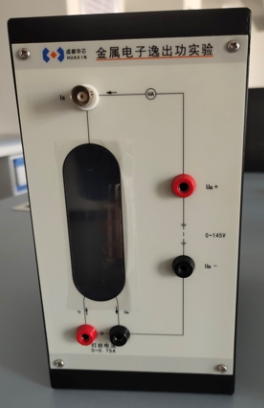
\includegraphics[width=\linewidth]{assets/实验仪器-金属电子逸出功.png}
    \caption{金属电子逸出功实验仪}
  \end{minipage}
  \hspace{1em} % 添加一点水平间距，防止图片紧贴
  \begin{minipage}[c]{0.45\linewidth}
    \centering
    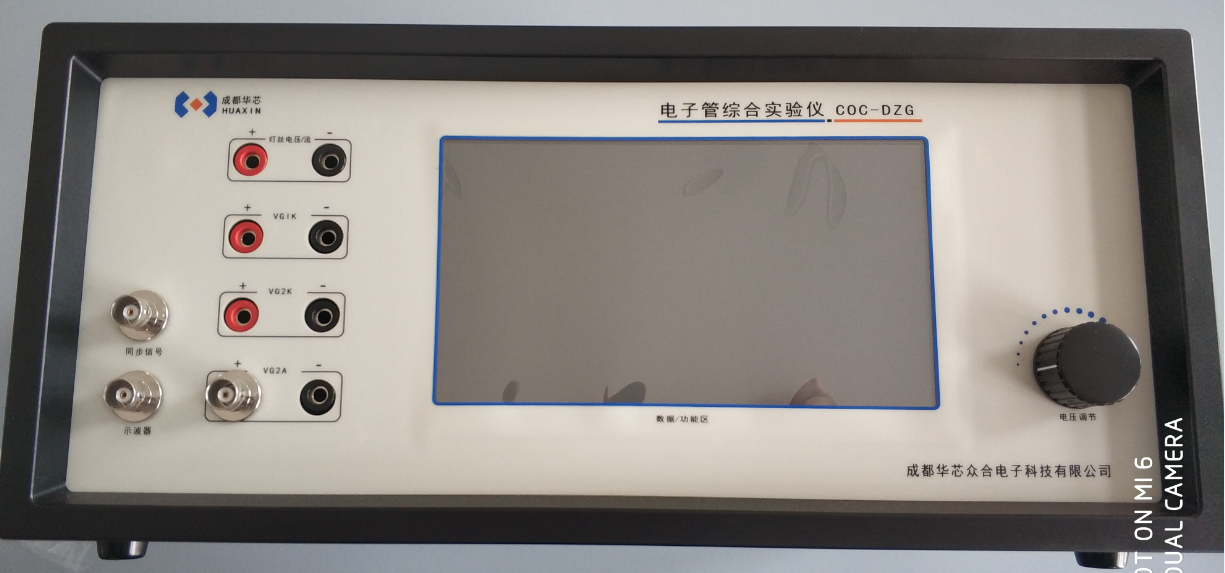
\includegraphics[width=\linewidth]{assets/实验仪器-电子管综合实验仪.png}
    \caption{电子管综合实验仪}
  \end{minipage}
\end{figure}


\section{实验原理}

\subsection{电子逸出功}
根据电子从金属表面逸出提供能量的方式不同，电子发射可以分为光电子发射、热电子发射、二次电子发射、场效应发射四种类型。本实验用加热金属，使热电子发射的方法测定金属的电子逸出功。
\subsection{热电子发射测量电子逸出功的原理}

热电子发射遵循查逊—杜什曼（Richardson-Dushman）公式 ：
\begin{equation}
I_0 = A S T^2 \exp\left({-\frac{e\varphi}{kT}}\right) \label{eq-rd}
\end{equation}

其中 $I_0$ 为热电子发射的零场电流强度 ；
   $A$ 为与阴极表面化学纯度有关的系数 ；
   $S$ 为阴极的有效发射面积 ；
   $T$ 为发射热电子的阴极绝对温度 ；
   $k$ 为玻尔兹曼常数 ；
   $e\varphi$ 为电子逸出功 。

原理上只要测出 $I_0$、$S$、$T$ 和 $A$，即可计算出逸出功。
但由于 $A$ 和 $S$ 难以直接测定，实验采用里查逊直线法。对公式 \ref{eq-rd} 两边除以 $T^2$ 并取对数得
% \begin{equation}
$$
\lg\left(\frac{I_0}{T^2}\right) = \lg(AS) - 5.04\times10^3 \varphi \frac{1}{T}
$$
% \end{equation}
此式表明 $\lg(I_0/T^2)$ 与 $1/T$ 成线性关系。如果以 $1/T$ 为横坐标，$\lg(I_0/T^2)$ 为纵坐标作图，由直线的斜率可求出电子的逸出电势 $\varphi$ 从而求出电子逸出功 $e\varphi$。这种数学处理的方法就叫里查逊直线法。

\subsection{零场电流的测量方法}

在热电子发射过程中，由于空间电荷产生的电场会阻碍电子飞向阳极 。为消除此影响需额外施加一加速电场 $E_a$，使电子一旦逸出就能迅速飞往阳极。但 $E_a$ 的存在会产生肖脱基效应，导致实测电流 $I_a$ 大于零场电流 $I_0$ 。它们的关系为
% \begin{equation}
$$
I_a = I_0 \exp\left({0.439\sqrt{E_a}/kT}\right)
$$
% \end{equation}
取对数得
\begin{equation}
\lg I_a = \lg I_0 + \frac{0.439\sqrt{E_a}}{2.30T} \label{eq-4}
\end{equation}
加速电场可近似为
$$
E_a= \frac{U_a}{r_1 \ln(r_2/r_1)}
$$
其中 $r_1$ 和 $r_2$ 分别为阴极和阳极的半径，$U_a$ 为阳极电压。代入式 \ref{eq-4} 得
% \begin{equation}
$$
\lg I_a = \lg I_0 + \frac{0.439}{2.30T}\sqrt{\frac{1}{r_1 \ln(r_2/r_1)}}\sqrt{U_a}
$$
% \end{equation}
由此可见，当阴极温度 $T$ 一定时，$\lg I_a$ 与 $\sqrt{U_a}$ 成线性关系 。通过作 $\lg I_a \sim \sqrt{U_a}$ 图线并延长至 $\sqrt{U_a}=0$ 处，其截距即为 $\lg I_0$，从而求得零场电流 $I_0$ 。


\section{实验内容和步骤}
\noindent
\begin{minipage}[t]{0.6\linewidth} % 左侧文字部分，占 65% 宽度
  % \begin{enumerate}[nosep, leftmargin=*] % nosep 消除所有垂直间隙
  \textbf{1.} 按照图1.2a连接好实验电路，接通电源。\\
  \textbf{2.} 调节理想二极管灯丝电流 $I_f$，在 0.6--0.7A 之间每隔 0.025A 进行一次测量。对于每一灯丝电流，预热 3--5 分钟，对应温度按照：$T = 900 + 1430 I_f$ 求得（如果阳极电流 $I_a$ 偏小或偏大，也可适当增加或降低灯丝电流 $I_f$）。\\
  \textbf{3.} 对每一灯丝电流，在阳极上依次加上 25V, 36V, 49V, 64V, 81V, 100V, 121V, 144V 电压，各测出一组阳极电流 $I_a$ 填入表1。
  % \end{enumerate}
\end{minipage}
\hfill
\begin{minipage}[t]{0.35\linewidth} % 右侧图片部分，占 30% 宽度
  \vspace{-10pt} % 确保图片与第一行文字对齐
  \centering
  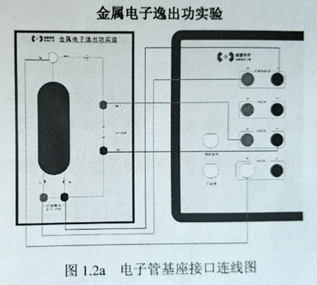
\includegraphics[width=\linewidth]{assets/图1.2a.png}
\end{minipage}

\newcolumntype{Y}{>{\centering\arraybackslash}X}
\begin{LabRecordTable}
  \centering
  \renewcommand{\arraystretch}{1.2}
  \caption{不同灯丝电流 $I_f$ 和阳极电压 $U_a$ 对应的阳极电流 $I_a$ 值}
  \label{table1}
  \setlength{\tabcolsep}{3.5pt}
  \begin{tabularx}{\textwidth}{c *{8}{Y}}
    \toprule
    & \multicolumn{8}{c}{$U_a$ / V} \\
    \cmidrule(lr){2-9}
    $I_f$ / A & 25 & 36 & 49 & 64 & 81 & 100 & 121 & 144 \\
    \midrule
    0.600 & & & & & & & & \\
    0.625 & & & & & & & & \\
    0.650 & & & & & & & & \\
    0.675 & & & & & & & & \\
    0.700 & & & & & & & & \\
    \bottomrule
    \multicolumn{9}{l}{\small 注：表中数据单位为 mA。}
  \end{tabularx}
\end{LabRecordTable}

\section{实验数据处理}
\begin{enumerate}
  \item 根据表 \ref{table1} 中的数据，作出 $\lg I_a \sim \sqrt{U_a}$ 图线（图 ?）。直线的截距即为对应关系式中的 $\lg I$，由此可得在不同阴极温度时的零场热电子发射电流 $I$。 
  \item 将图 ? 中各温度下的直线截距值填入表 \ref{table2} ，作出 $\lg (I/T^2) \sim 1/T$ 图线（图 ?）。根据直线斜率，求电子逸出电势及金属钨的电子逸出功。并与公认值 4.54 eV 比较，求测量相对误差。 
\end{enumerate}

\begin{table}[htbp]
  \centering
  \caption{$\lg(I/T^2)\sim 1/T$ 图线相关数据}
  \label{table2}
  \begin{tabularx}{\textwidth}{c *{5}{Y}}
    \toprule
    $I_f$ / A & & & & & \\
    \midrule
    $T$ / K & & & & & \\
    $\lg I$ / mA & & & & & \\
    $1/T$ / $10^{-4}\,\mathrm{K}^{-1}$ & & & & & \\
    $\lg(I/T^2)$ & & & & & \\
    \bottomrule
  \end{tabularx}
\end{table}

\section{实验的分析和总结}

\newpage

% \insertRawDataPage
\insertSignedDataPage

\end{document}
